\documentclass[11pt,aspectratio=169]{beamer}
\usepackage[T1]{fontenc}
\usepackage[utf8]{inputenc}
\usepackage{lmodern}
\usepackage{booktabs,tabularx}
\usepackage{graphicx}
\usepackage{amsmath, amssymb, amsfonts, amsthm, bbm}
\usepackage[
    natbib=true,
    bibencoding=inputenc,
    bibstyle=authoryear-ibid,
    citestyle=authoryear-comp,
    maxcitenames=3,
    maxbibnames=10,
    useprefix=false,
    sortcites=true,
    backend=bibtex
]{biblatex}
\AtBeginDocument{\toggletrue{blx@useprefix}}
\AtBeginBibliography{\togglefalse{blx@useprefix}}
\setlength{\bibitemsep}{1.5ex}
\addbibresource{References.bib}

%\usepackage{enumitem}
\usepackage{hyperref}
\hypersetup{
    colorlinks=true,
    linkcolor=black,
    anchorcolor=black,
    citecolor=black,
    filecolor=black,
    menucolor=black,
    runcolor=black,
    urlcolor=black}

\DeclareMathOperator{\argmax}{arg\,max}

%Theorem
\newtheorem{assumption}{Assumption}
\newtheorem{proposition}{Proposition}
%\newtheorem{definition}{Definition}


\begin{document}
\mode<presentation>{	
    \setbeamertemplate{navigation symbols}{}
}

\title{Topics in Behavioral Decisons in Finance}
\date{Discussion by Christian Hilpert\\ \today}
\begin{frame}
    \titlepage
\end{frame}


\begin{frame}{4. Applications and Limitations of CPT}
Three sample applications to highlight:
    \begin{enumerate}[i)]
        \item how to apply CPT \\
        \item interesting applications on ???\\
        \item key limitations of CPT\\
    \end{enumerate}
  
\end{frame}


\begin{frame}{4.1. Azevedo and Gottlieb (2012,JET) }
    \begin{itemize}
        \item What happens in strategic and market environments? \medskip
        \item Consider monopolistic insurer, CPT customer\medskip
        \begin{itemize}
            \item $\Rightarrow$ Monopolist can charge any arbitrarily large price ploicy features unbounded gains or losses with probability approaching zero.\medskip
            \item $\Rightarrow$ Counterintuitive: insurance raises risk; no solution to firm's problem\medskip
        \end{itemize}
        \item  For any insurance policy, there is always another policy that makes both the firm
        and consumers simultaneously better off. \medskip
        \item  If consumer's wealth is bounded, the insurer can extract all wealth with probability approaching one. (Bertrand competition, no equilibrium exists) \medskip
    \end{itemize}
\end{frame}

\begin{frame}{4.1. Azevedo and Gottlieb (2012,JET)}
 Additionally,
    \begin{enumerate}[i)]
        \item  individuals pay arbitrarily large amounts for lotteries with finite expected value \\
        \item  individuals refuse all actuarially fair gambles\\
    \end{enumerate}
    Case\begin{enumerate}[(i)]
        \item  implies no equilibrium if supply is endogenous. \\
        \item  rules out simultaneous risk-seeking and aversion. \\
    \end{enumerate}
(why we use CPT in the first place)
\end{frame}

\begin{frame}{Model}
    \begin{itemize}
        \item Gamble: $\mathcal{L} =(g,p;L,1-p), g \geq 0, -L\leq 0 $\\
        \item CPT: $V(\mathcal{L} )= w^{+}(p)v(g)-\lambda w^{-}(1-p)v(L).$\\
$w^{+},w^{-}:[0,1] \rightarrow [0,1]$,   \quad $ v:\mathbb{R}_{+} \rightarrow \mathbb{R}$\\
        \item Assumption:
$v$ is continuous, strictly increasing ,$v(0)=0$\\
$w^{+},w^{-}$ are continuous, strictly increasing,\\
\qquad  $w^{+}(0)=w^{-}(0)=0$; $w^{+}(1)=w^{-}(1)=1$\\
        \item Risk-neutral firm designs $\mathcal{L}$, perfect information, monopolist.\\
        \item profit :$\pi(\mathcal{L})=(1-p)L-pg$\\
$\Rightarrow$ maximise expected profit s.t. $V(\mathcal{L})\geq 0$ (participate)\\
    \end{itemize}
\end{frame}

\begin{frame}{4.1. Azevedo and Gottlieb (2012,JET)}
    \begin{proposition}
    suppose either :
    \begin{enumerate}[(1)]
        \item $\lim_{p \to 0} w^{+}(p)v(\frac{1}{p})=\infty  $ ,or\\
        \item $\lim_{p \to 0} w^{-}(p)v(\frac{1}{p})=0  $\\
    \end{enumerate}
    Then, for any $K_1,K_2$, there exists a lottery $\mathcal{L}$ 
    s.t. $\pi(\mathcal{L}) \geq K_1$ and $V(\mathcal{L}) >v(K_2)$\\
    In particular, $\prod (V)=\infty.$\\
    \end{proposition}
    \hspace*{\fill} \\
\textbf{Proof:}\\
\begin{itemize}
    \item Consider the lottery$ (\frac{1}{p},p;\frac{1+\pi}{1-p},1-p)$.\\
    \item Assum(1) $\Rightarrow \mathbb{E} [\cdot]= (1- p)\frac{1+\pi}{1-p}-\frac{1}{p}p =\pi  $\\
and $\lim_{p \to 0} w^{+}(p)v(\frac{1}{p})- \lambda w^{-}(1-p)v(\frac{1+\pi}{1-p})  $
$\geq \lim_{p \to 0} w^{+}(p)v(\frac{1}{p})- \lambda v(1+\pi)$\\
$\Rightarrow $  arbitrarily high utility, profit $\pi >0$.  
\end{itemize}
\end{frame}

\begin{frame}
    \begin{itemize}
        \item Assum(2). Consider:$ (\frac{u}{p},p;\frac{\pi+u}{1-p},1-p), u,\pi \geq 0.$\\
    $ \mathbb{E} [\cdot]= (1- p)\frac{\pi+u}{1-p}-\frac{u}{p}p =\pi  $\\
    \item CPT:$ w^{+}(p)v(\frac{u}{p})- \lambda w^{-}(1-p)v(\frac{u+\pi}{1-p})  $\\
    \item the limit:\\
 $\lim_{p \to 1}w^{+}(p)v(\frac{u}{p})- \lambda w^{-}(1-p)v(\frac{u+\pi}{1-p})$\\
    $=v(u) -\lambda \lim_{p \to 0} w^{-}(p)v(\frac{\pi+u}{p})=v(u)$\\
    \item $\Rightarrow $  any profit $\pi \geq 0$ ,any utility $v(u) \in [0,v(\infty))$,$p$ close to $1$.
\end{itemize}
\end{frame}

\begin{frame}{4.1. Azevedo and Gottlieb (2012,JET)}
\textbf{Interpretation:}
\begin{enumerate}[(1)]
    \item Cond.1: lottery, large sum $\frac{1}{p}$ with low $p$,and $0$ else\\
    \begin{itemize}
        \item Expected value is one, gain $\frac{1}{p}$ grows unboundedly as $p \rightarrow 0$.\\
        \item     Customer pays arbitrary amounts for expected value of 1. \medskip
        \item $\Rightarrow$ firm infinite expected profits, gives arbitrarily large certainty equivalents. \medskip
    \end{itemize}
    \item Cond.2: large loss $\frac{1}{p}$ utility\\
    \begin{itemize}
        \item Expected payment $=-1$,unbounded loss $\frac{1}{p}$\medskip
        \item $\Rightarrow$ arbitrarily small risk premium. \medskip
        \item Customer accepts negative expected payoff for arbitrarily small prices, firm again has infinite profits,customer infinite utility.\\
        \item Catastrophe bonds below fair price.
    \end{itemize}
\end{enumerate}
\end{frame}

\begin{frame}{4.1. Azevedo and Gottlieb (2012,JET)}
    \begin{itemize}
        \item Under both 1 and 2: \\
        firm has infinite profits for any lottery, there always is a better one for both firm and customers as $p \rightarrow 0$.\\
        \item Additionally, $v(x)=x^\alpha, 0<\alpha \leq 1$.\\
        \item $\Rightarrow$ homogeneous of degree $\alpha$.\\
        \item For any $\mathcal{L} =(g,p;L,1-p) $ and 
        $c\mathcal{L} =(cg,p;cL,1-p) $, \\
        $V(c\mathcal{L}) = c^\alpha V(\mathcal{L}),  c>0 $.\\
        \item $\Rightarrow v(c\mathcal{L}) \geq  V(\mathcal{L})$.\\
        \item If individual accepts $\mathcal{L}$, he must also accept $c\mathcal{L}$.\\
        \item $\Rightarrow$ firm profit $\pi \rightarrow c\pi$.\\
        \item Hence, if seller can obtain a positive profit, it can obtain any positive profit.
    \end{itemize}
\end{frame}

\begin{frame}{4.1. Azevedo and Gottlieb (2012,JET)}
    \begin{itemize}
        \item The choice of $\omega $ empirically does not matter.\\
        \item all estimated forms of $\omega$ satisfy our conditions.\\
        \item adding a reference point $r\neq 0$ does not change anything.\\
        \item Competition $\grave{a}  la$ Bertrand $\Rightarrow$ no equilibrium. \\
        \item Heterogeneity does not matter for result.\\
        \item Wealth constraints $B>0$ bounds profits, rest remains\\
        \item one solution: global + local utility (next lecture)
    \end{itemize}
\end{frame}

\begin{frame}{4.2. Barberis (2012,MS)}
    \begin{itemize}
        \item Why do people gamble? \medskip
        \item Why can CPT shed light? Loss acersion? \\\medskip
        Even probabilityies $\Rightarrow$ unappealing  $ \neq $ lottery
        \item General point: time inconsistency.\\
        \item shows:
        \begin{itemize}
            \item CPT agent gambles for many parameters, no skewness and zero or negative expected value.  \medskip
            \item CPT implies time inconsistency.  \medskip
            \item 50/50 bets.
            \item Inityal plan: play if winning, quit on lossing.\\
             isolated bet unattractive,\\
            c???? bets good:  low loss, high ???,\\
              probability weighting: expected value: $p(5*winning)$\\
              $\frac{1}{5}^5=\frac{1}{32} \Rightarrow $ low, overweighted\\
              after a winning bets:$\frac{1}{2} \Rightarrow$ underweighted\\
              $\Rightarrow $ preference change over time.
        \end{itemize}
    \end{itemize}
\end{frame}


\begin{frame}{4.2. Barberis (2012,MS)}
    \begin{itemize}
        \item predicts heterogeneity in gambling behavior:\\
        \begin{enumerate}
            \item naive: plans, deviate from plan.\\
            \item sophisticated:knows time incosistency, cannot commit\\
            $\Rightarrow$ predicts losing
            \item sophisticated with commitment\\
            $\Rightarrow$ predicts behaviors, sticks with (eg: only takes limited cash).\\
        \end{enumerate}
    \end{itemize}
\end{frame}


\begin{frame}{Model:}
    \begin{itemize}
    \item same as before:
        \begin{equation}
        v(x) = \begin{cases}
            x^\alpha  &  \text{for} \quad x \geq 0,\\
            -\lambda (-x)^\alpha & \text{for} \quad x<0,
            \end{cases}
        \end{equation}\medskip
        and \\
        {\centering $ \omega(p)=\frac{p^\delta }{(p^\delta + (1-p)^\delta)^{\frac{1}{\delta}}} $\\

        }
        \hspace*{\fill} \\ 
    \item $ \alpha \in (0,1], \lambda>1,  \delta \in (0,1) $\\ \medskip
    \item $T+1$ dates,$t=0,1,...,T.$\\ \medskip
    \item at $t=0$, $50:50$ bet: gain /lose $h$.\\
    at any time bet, if declines once, game is over.
    \end{itemize}
\end{frame}

\begin{frame}{4.2. Barberis (2012,MS)}
    Take $T=5$ for example
        \begin{itemize}
            \item  Binomial Tree Representation \medskip
        \end{itemize}
        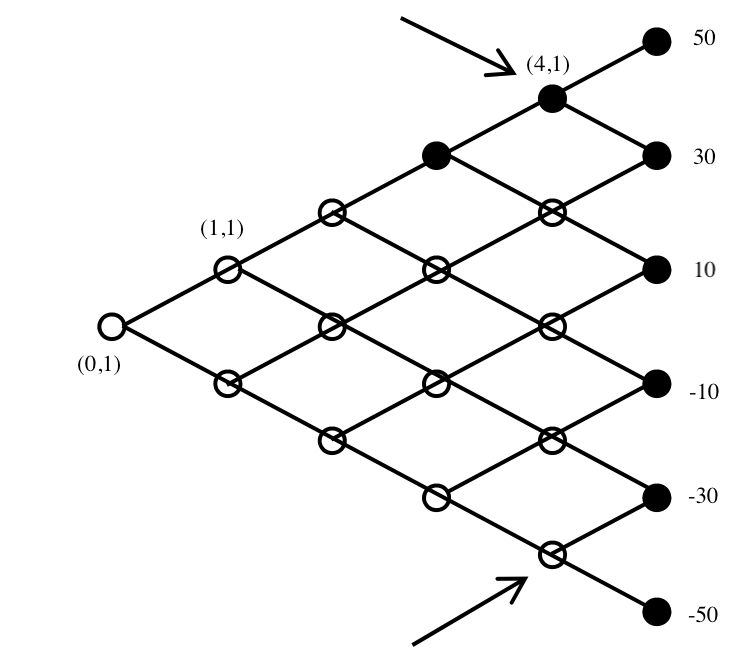
\includegraphics[width = 0.5\textwidth]{fig2.png}\\
    (black: no gamble; white: gamble)
    \end{frame}

\begin{frame}{Binomial Tree Representation}
    \begin{itemize}
        \item each node $(t,j)$.  \medskip
        \item $t \in {0,\ldots ,T}$ \medskip
        \item $ j \in {1,\ldots,t+1}$, how far down:$j=1$ top node.\medskip
        \item Assume: $r=0$,CPT of whole evening
        \item  time inconsistency:\\
        $(4,1)$: initial probability $\frac{1}{2}$ : gain 50 or down 30  $\Rightarrow$ gamble\\
        \item if actually at $(4,1)$:\\
        $v(40) \geq v(50)\omega (\frac{1}{2})+v(30)(1-\omega (\frac{1}{2})) \Rightarrow$ usually exit. \\
        $\Rightarrow v(40)-v(30) \geq (v(50)-v(30))\omega (\frac{1}{2})   $;  holds for all $\alpha, \delta \in (0,1)$.\\
        \item similar: initial plan: stop at (4,5), not keep gambling\\
    \end{itemize}
\end{frame}

\begin{frame}{4.2. Barberis (2012,MS)}
    \begin{itemize}
        \item general description for fixed strategies $s \in S(0,1)$\\
        \item $\tilde{g_s} $ : the accumulated winnings or losses\\
        \item $\tilde{g_s} \backsim (30,\frac{7}{32};10,\frac{9}{32};-10,\frac{10}{32};-30,\frac{5}{32};-50,\frac{1}{32} )  $\\
        \item $\Rightarrow \max_{s \in S(0,1)} V(\tilde{g_s})$\\
        \item generally no analytically solution.\\
    \end{itemize}
\end{frame}

\begin{frame}{4.2. Barberis (2012,MS)}
\textbf{Numerical analysis} \\  
\textbf{naive agent} 
    \begin{itemize}
        \item many parameters enter, that is $V(\tilde{g_s})>0 $ \medskip
        \item deviations for naive agent: $(\alpha,\delta,\lambda)=(0.95,0.5,1.5)$
    \end{itemize}
    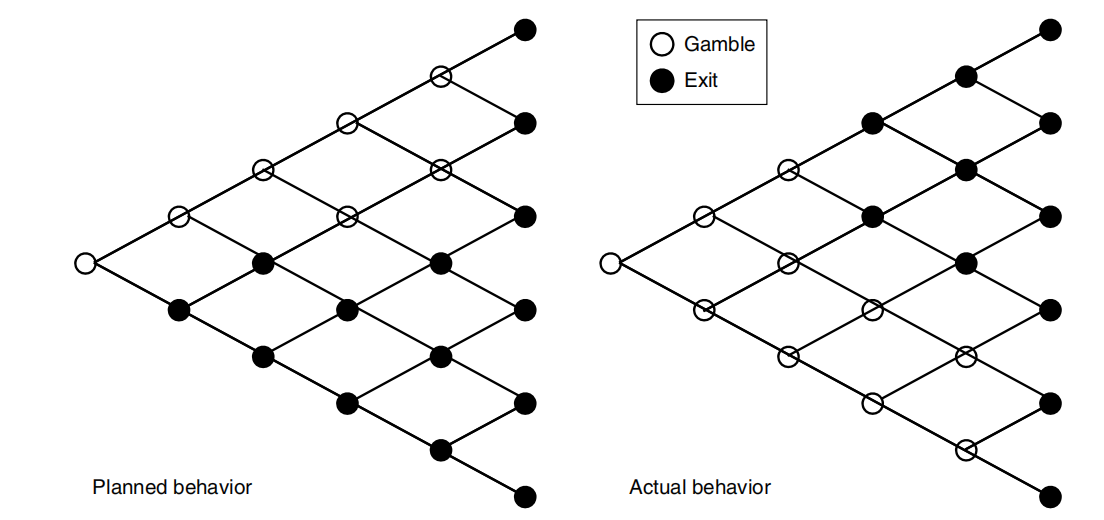
\includegraphics[width = 0.7\textwidth]{fig3.png}\\
\end{frame}

\begin{frame}{4.2. Barberis (2012,MS)}
    \begin{itemize}
        \item mostly: plan a "loss exit" plan \medskip
        \item some: plan a "gain exit" plan \\
        \item probility weighting most important \medskip
    \end{itemize}
\textbf{sophisticated without commitment}
    \begin{itemize}
        \item aware of time incosistency\medskip
        \item  uses backward induction
        \item node $(t,j),t \in [0,T-1]$\\
        $V(\tilde{g_{t,j}})>v(h(t+2-2j)) $;\\
         $v(h(t+2-2j))$: leave immediately; \\
        $ V(\tilde{g_{t,j}})  $: the value of continuing to gamble.\\
        $\Rightarrow$ rarly enters casino; only if  $\alpha,\lambda $ small,$\delta$ large\\
    \end{itemize}

\end{frame}

\begin{frame}{4.2. Barberis (2012,MS)}
    \textbf{sophisticated with commitment}
    \begin{itemize}
        \item same as naive agent, but goes through \medskip
        \item no time inconsistency \medskip
        \item want to gamble in the region of losses\\
        \item take a small amount of cash
    \end{itemize}
\end{frame}

\begin{frame}{4.2. Barberis (2012,MS)}
    \textbf{Proposition}    
    \begin{itemize}
        \item An EU maximiser stops all Brownian motions with  ??? and small variance at every wealth level where his utility function is of expanetial growth.\\ 
        \item $\Rightarrow$ ever ???? stops immediately.\\
    \end{itemize}
    \textbf{Some Implications}    
    \begin{itemize}
        \item ??? ,infinite horizon casino \medskip
        $dX_t=\mu dt+ \sigma dW_t, \mu(x)\equiv \mu <0, \sigma(x)=\sigma >0 $\\
        $\Rightarrow $ gamble utility ??? , appears almost  ???.\\
        \item American option: $\max (X_t-\mu,0)$ if ex. at time t.\\
        $dX_t=X_t(\mu dt+ \sigma dW_t) $
        \item $\Rightarrow $ never exerise real option, even if $X_0 > \mu$ \medskip
        \item no disposition ????
    \end{itemize}
    \textbf{Constraints}  
    \begin{itemize}
        \item naive \medskip
        \item probability weighting dominant. \medskip
    \end{itemize}
\end{frame}

\end{document}
